
\hypertarget{2008}{}
\section{Versions released in 2008 (14)}
\index{What is New?!2008}
\subsection*{2.1.1.6 (Nov/17/2008)}
\begin{itemize}
  \item Bug(s) fixed:
    \begin{itemize}
      \item All fonts of \textit{Tools/Markup} interface are now visible.
    \end{itemize}
  \item The \textit{Application options} was a bit reworked.
  \item Due to focus changes behavior in the latest Tinn-R
    version (2.1.1.5), the focus control button (options toolbar )
    will be not enabled if Rterm is running. In this case, the focus
    will be always returned to the interface (editor or Rterm) that
    has the prior focus before all send/control options.
\end{itemize}


\subsection*{2.1.1.5 (Nov/12/2008)}
\begin{itemize}
  \item Bug(s) fixed:
    \begin{itemize}
      \item Related to \textit{Inverse DVI Search};
      \item Focus control working with dual monitor.
    \end{itemize}
  \item The latest \htmladdnormallink{Windows installer}
    {http://txt2tags-win.sourceforge.net/index.html.pt-br}
    version is 2.3. Therefore, it was necessary to adapt Tinn-R to
    work with the interpreter Phyton for Windows (python.exe) and
    the python script to make the conversion (txt2tags). The current
    version of Txt2tags is 2.5.
  \item To install and configure the necessary resources follow these simple steps:
    \begin{enumerate}
      \item Download and install the interpreter
        \htmladdnormallink{Python}{http://www.python.org/download/};
      \item Download and unzip
        \htmladdnormallink{Txt2tags}{http://txt2tags.sourceforge.net/}
        inside any folder anywhere in your computer;
      \item Inside of Tinn-R, go to 'Options/Application/Processing/Txt2tags'
        and inform the necessary: parameters (\textit{-t} is the default)
        and the paths of interpreter (\texttt{python.exe}) and the
        converter (\texttt{txt2tags python script});
      \item It is enough to use these nice tools in the Tinn-R project.\\


        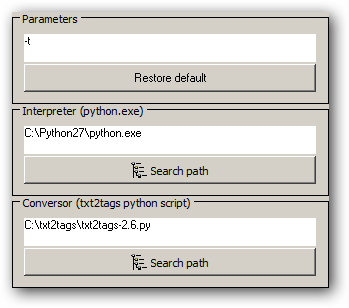
\includegraphics[scale=0.50]{./res/txt2tags.png}
    \end{enumerate}
\end{itemize}


\subsection*{2.1.1.4 (Nov/10/2008)}
\begin{itemize}
  \item Bug(s) fixed:
    \begin{itemize}
      \item Closing the applicative if \textit{Rterm} is runnig (random bug).
      \item \textit{Options: return focus after sending to R}:
        \begin{itemize}
          \item If in editor, the focus shifts back after sending to R;
          \item If in \textit{Rterm} (or \textit{Rgui}), the focus does not
            jump back to editor when you press return: \texttt{ENTER}
            (prompt line), or \texttt{CTRL + ENTER} (any prior line).
        \end{itemize}
    \end{itemize}
  \item The \textit{Options/Application/Main} menu has a new \texttt{Dock} page. It
    enables the user to fix any possible problem related to visualization
    (\textit{dock/hide}) and layout of the \texttt{Tools and Rterm}
    interfaces.
  \item The resources of \textit{Rterm} interface were extended:
    \begin{itemize}
      \item All resources available enabling the control of \RR{} are now also
        available to \textit{IO} and \textit{Log} interfaces: print content,
        plot, list names, etc;
      \item {To all options enabling the control of R, THE FOCUS WILL BE MAINTENED
          IN THE CURENT WORK INTERFACE Editor or IO, DISREGARDING the Options:
          return focus to editor after send/control \RR{} (toogle)}.
    \end{itemize}
  \item Rterm interface and debug package:
    \begin{itemize}
      \item Changes were made to the debug package (1.0.2) on the message system
        (\textit{stdout} and \textit{stderr}). The default option is not
        compatible with Rterm interface implementation.
      \item The best way to make it compatible again is to add the option below
        in the Rprofile.site file:

        \begin{Scode}
          options(debug.catfile = 'stdout')
        \end{Scode}

    \end{itemize}
\end{itemize}


\subsection*{2.1.1.3 (Nov/04/2008)}
\begin{itemize}
  \item Bug(s) fixed:
    \begin{itemize}
      \item \textit{Application options/Appearance} when the user
        select \textit{Cancel}.
      \item \textit{R control: packages (both: Load and Remove)} and
        \textit{Rterm interface}.
      \item Rterm interface under package \textit{debug} of Mark V.
        Bravington when the user type \texttt{qqq()} to quit the debugger.
    \end{itemize}
  \item The interface \textit{Go to line number} was a bit reworked.
\end{itemize}


\subsection*{2.1.1.2 (Oct/20/2008)}
\begin{itemize}
  \item The appearance of the main menu and all pop-up menus were improved.
  \item Now Tinn-R is able to perform \texttt{inverse DVI search}. It is
    only necessary to set  the path of the binary of Tinn-R and the parameter
    for file and line in your DVI previewer.
    For example, using the YAP of Miktex, the necessary configuration will be
    (assuming the default Tinn-R path):

    \begin{footnotesize}
      \begin{verbatim}
        C:\Tinn-R\bin\Tinn-R.exe "%f;%l"
      \end{verbatim}
    \end{footnotesize}


    Be sure that there is not space between the parameters \%f(related to file)
    and \%l(related to line).

    Inside Tinn-R (\textit{Options/Application/Processing/Latex/DVI}) it is necessary
    to add the compilation Miktex parameter: latex -c-style-errors \texttt{--src-specials}.
    Tinn-R can do it automatically with the option \textit{Restore default}. Now, it is:

    \begin{footnotesize}
      \begin{verbatim}
        latex -c-style-errors --src-specials
        and
        bibtex --src-specials
      \end{verbatim}
    \end{footnotesize}

\end{itemize}


\subsection*{2.1.1.1 (Oct/15/2008)}
\begin{itemize}
  \item Bug(s) fixed:
    \begin{itemize}
      \item Bugs of the version 2.X.X.X (prior of this version) related to the
        \textit{R/Configure/Temporary (current session)} and
        \textit{R/Configure/Permanent (Rprofile.site)} were fixed.
      \item A bug related to the \textit{Rterm} interface with incomplete instructions
        ('+') was fixed. An undesirable carriage return after the '+ CR', the
        origin of the bug, was eliminated.
      \item A bug related to the status (show/hide) of the toolbars \textit{Spell}
        and \textit{Search} when closing and starting the application was fixed.
    \end{itemize}
  \item Version restricted to pre-release testers.
  \item The way Tinn-R creates the variable \texttt{.trPaths} was changed.
    Now it is automatic. It was posted on
    \htmladdnormallink{Tinn-R forum}{https://sourceforge.net/forum/forum.php?thread\_id=2219532\&forum\_id=481901}
    by KeithJ (keith\_jewell) - 2008-09-15 16:00. It is very useful in
    laboratories where most users have their own account but use the
    same computer. Now it is not necessary to adapt the file
    \texttt{Rprofile.site} for each user and \RR{} session any more. Many thanks
    to \texttt{keith Jewell} for the nice suggestion.

    \begin{footnotesize}
      \begin{verbatim}
        .trPaths <- paste(paste(Sys.getenv('APPDATA'), '\\Tinn-R\\tmp\\', sep=''),
        c('', 'search.txt', 'objects.txt', 'file.r', 'selection.r', 'block.r', 'lines.r'), sep='')
      \end{verbatim}
    \end{footnotesize}

  \item The option \textit{Save/Load} workspace to the Rterm interface was added.
    Many thanks to \texttt{Maria Concei��o} for the suggestion.
  \item The \textit{Tools} and \textit{Rterm} interfaces were reworked and now both
    are dockable. It makes the interface flexible and user customizable. Many thanks
    to \texttt{Thomas Petzoldt} for the suggestion.
  \item A new option was added to the \textit{Options}: \texttt{max.deparse.length
      (echo=TRUE)}. It is used if \texttt{echo is TRUE} and gives the maximal number
    of characters output for the deparse of a single expression.
  \item The weblinks links of the menu \textit{Web} were all updated.
  \item In order to attend to the request of some users, the menu
    (and related pop-up menu) \textit{Edit} go back to the project interface with
    a new implementation. Due to the large frequency of the use of class SynEdit
    (editor, editor split, IO, Log, etc), the action will be apllied in the active
    (selected) instance of the class SynEdit.
  \item The \textit{font} of the \textit{Rterm} interface is now updated after changes
    to \textit{Options/Editor/Display/Font}.
\end{itemize}


\subsection*{2.0.0.7 (Sep/04/2008)}
\begin{itemize}
  \item Bug(s) fixed:
    \begin{itemize}
      \item A bug related with the package \textit{Rterm} interface was fixed.
    \end{itemize}
\end{itemize}


\subsection*{2.0.0.6 (Aug/21/2008)}
\begin{itemize}
  \item Bug(s) fixed:
    \begin{itemize}
      \item A bug related to the package \textit{Matrix} was fixed. Many
        thanks to \texttt{Frank} for point it out!
    \end{itemize}
  \item The \textit{Rterm} interface can be used to connect with \RR{} as
    a remote server. Sorry, it is already running, but it was not finished yet!
\end{itemize}


\subsection*{2.0.0.5 (Aug/17/2008) - pre-release}
\begin{itemize}
  \item Bug(s) fixed:
    \begin{itemize}
      \item A bug related to the function \textit{debug(base)} was fixed.
        Many thanks to \texttt{Steven} for pointing it out!
    \end{itemize}
\end{itemize}


\subsection*{2.0.0.4 (Aug/12/2008) - pre-release}
\begin{itemize}
  \item Small corrections and adaptations suggested by testers.
    Many thanks to \texttt{Steven}.
  \item The \RR{} history now stores up to 100 instructions.
\end{itemize}


\subsection*{2.0.0.3 (Aug/05/2008) - pre-release}
\begin{itemize}
  \item Version 2.0.0.2 (Jul/23/2008) was released to some selected
    users for tests; it was the lastest version compiled under the IDE
    \texttt{Delphi 7} of Borland.
  \item This version, and from now on, all versions will be compiled under
    the IDE \texttt{Code Gear 2007}, the latest of Borland.
\end{itemize}


\subsection*{2.0.0.2 (Jul/23/2008) - pre-release}
\begin{itemize}
  \item Small corrections suggested by pre-release testers. Many thanks
    to \texttt{John}, \texttt{Steven} and \texttt{Frank} for the tests
    and suggestions.
  \item This version, unlike 2.0.0.1, is fully compatible with the very
    useful package \textit{debug} (of Mark Bravington). It remains an
    unsolved problem to submit, when debuging, an external script with
    incomplete line, like the one below:

    \begin{Scode}
      plot(rnorm(1e2), main = 'It will cause error!')
    \end{Scode}

\end{itemize}


\subsection*{2.0.0.1 (Jul/22/2008) - pre-release}
\begin{itemize}
  \item Version restricted to pre-release testers.
  \item The structure of the \textit{ini} and the
    \textit{routine of initialization} were deeply reworked:
    \begin{itemize}
      \item The old backups \texttt{will not be compatible anymore
          with this one and future versions};
      \item When used for the first time, this version will try to
        recognize almost all prior user preferences.
    \end{itemize}
  \item A new folder, \texttt{bkp}, was added to the ini files structure.
    It contains all backups of all prior user preferences not
    (or partially) compatible with the new versions. The control of all
    default resources are now individual, i.e: \textit{custom},
    \textit{data}, \textit{latex}, \textit{shortcuts} and \textit{syntax}.
  \item The \textit{R explorer} functionality was reworked:
    \begin{itemize}
      \item The functions (\texttt{trObjSearch} and \texttt{trObjList}) were
        reworked. These functions are distributed with the package svMisc
        ($>$= 0.9.40) of Philippe Grosjean;
      \item To make the \RR{} interface cleaner, a new variable \texttt{.trPath}
        is used as additional parameter to the two functions above. It will
        avoid a long string like\\
        \footnotesize{\textit{path="C:/Documents and settings/User/Application Data/Tinn-R/Tmp/..."}}\\
        to Windows XP or \\
        \footnotesize{\textit{"C:/Users/jcfaria/AppData/Roaming/Tinn-R/tmp/..."}}\\
        on Windows Vista;
      \item The \RR{} object \texttt{.trPath} is a \textit{list} described below:

        \begin{Scode}
          .trPath <- list(
          Tmp = 'C:/Users/jcfaria/AppData/Roaming/Tinn-R/tmp/',
          Search = 'C:/Users/jcfaria/AppData/Roaming/Tinn-R/tmp/search.txt',
          Objects = 'C:/Users/jcfaria/AppData/Roaming/Tinn-R/tmp/objects.txt',
          File = 'C:/Users/jcfaria/AppData/Roaming/Tinn-R/tmp/file.r',
          Selection = 'C:/Users/jcfaria/AppData/Roaming/Tinn-R/tmp/selection.r',
          Block = 'C:/Users/jcfaria/AppData/Roaming/Tinn-R/tmp/block.r',
          Lines = 'C:/Users/jcfaria/AppData/Roaming/Tinn-R/tmp/lines.r'
          )
        \end{Scode}

      \item The best way to set the variable \texttt{.trPath} inside of \RR{}
        is using the options: \texttt{R/Configure/Temporary} or
        \texttt{R/Configure/Permanent}, both can be found in the main menu
        of Tinn-R \texttt{R/Configure};
    \end{itemize}

  \item The options to send \textit{File}, \textit{Selection}, \textit{Block}
    and \textit{Lines to end page}, were reworked:
    \begin{itemize}
      \item The objective was to maintain the \RR{} interface cleaner, thus
        avoiding long strings;
      \item All above are also dependent on the variable \texttt{.trPath};
      \item As already noted, the best way to set the variable
        \texttt{.trPath} inside \RR{} is using the options:
        \texttt{R/ Configure/ Temporary} or \texttt{R/ Configure/Permanent}.
        Both can be found in the main menu of Tinn-R \texttt{R/Configure}
    \end{itemize}
  \item The source code of Tinn-R was deeply reworked. The aim was to
    maintain the prior user knowledge, the stability, and the structural
    simplicity, but add more flexibility and power to the GUI, mainly
    associated with the new \texttt{Rterm} interface. The \textit{IO}
    and \textit{Log} interfaces are instances of the class synEdit:
    \begin{itemize}
      \item \texttt{IO}: the aim was to add flexibility and power, i.e.,
        joining the power of synEdit (editor) and the functionality of a
        common console. All prior user knowledge of the resources associated
        with the editor were preserved: marks, shortcuts, syntax, match
        brackets, tips, code completion, data completion, etc;
      \item \texttt{Log}: has two basic objectives:
        \begin{enumerate}
          \item To make the \textit{IO} interface cleaner;
          \item To avoid synchronization difficulties with the inter
            process communication (IPC) called \textit{pipe} in use.
        \end{enumerate}
      \item The shortcuts and the pop-up menu makes it easy to change among the
        interfaces: \textit{Editor}, \textit{IO} and \textit{Log}:
        \begin{enumerate}
          \item The common Windows shortcut \texttt{CTRL + TAB} changes
            the active page (IO-Log).
          \item Any prior line can be sent another time by just placing
            the cursor anywhere on and typing: \texttt{CTRL + ENTER};
        \end{enumerate}
      \item The last line of the \textit{IO} interface (the prompt) has
        special features:
        \begin{enumerate}
          \item It has some restrictions for edition and navigation;
          \item \texttt{ALT+DOWN} and \texttt{ALT+UP} are the shortcuts
            (prior/later) for command history. Both are continuous,
            cyclic and have a 50 lines limit (we think it is sufficient,
            but if necessary it can be increased to 100 or more).
        \end{enumerate}
    \end{itemize}
  \item When more than one recognized instance of \RR{} is running the
    priority order is:
    \begin{enumerate}
      \item Rterm;
      \item Rgui;
      \item Rserver (remote);
    \end{enumerate}
  \item The use of the clipboard as IPC was removed for all. It was an
    old request of users to avoid conflict with other application, mainly
    with the \texttt{Open Office} suit.
  \item The communication with \texttt{Rterm} is more specific and efficient
    than with \texttt{Rgui}. Therefore, it will receive more attention from
    the developers from now on. The interface with \textit{Rterm} is not
    finished yet, but it is running nicely...
    \begin{itemize}
      \item If some problem happens: press ENTER;
      \item If it is not solved, type anything and press ENTER;
      \item If it still not solved, sorry: close and restart the
        \textit{Rterm} instance;
      \item Remember: it is not finished yet!
    \end{itemize}
  \item The TCP/IP resources now are used only with two objectives:
    \begin{enumerate}
      \item \texttt{Local}: to make the \textit{Rterm} and
        \textit{Rgui} console cleaner;
      \item \texttt{Remote}: for all: send, control and output.
    \end{enumerate}
  \item A new interface \textit{Work expl.} was added to the
    \textit{Tools} interface. It will always show the folder and
    files of the latest file opened.
    It is simpler and has complementary resources to the \
    textit{Windows expl.} interface.
  \item The menu \textit{Edit} and associated pop-up menu were
    removed, but, all the functionality was preserved under shortcuts.
    To set the preferences see \textit{Options/Editor/Keystrokes}.
  \item The \textit{Tools} interface was a bit reworked and has new
    resources.
  \item The main menu was a bit reworked.
  \item The interface of the application options was a bit reworked.
  \item Due to new resources (\textit{IO} interface related with
    \texttt{Rterm}) the default shortcuts to view \textit{Line numbers}
    and \textit{Special characters} were changed to \texttt{CTRL + ALT + L}
    and \texttt{CTRL + ALT + K} respectivelly. Now \texttt{CTRL + L} clears
    the \textit{IO} and \textit{Log} interface, like \texttt{Rgui}.
  \item The main component synEdit was updated to the latest stable
    version and minor bugs were fixed.
  \item The descriptions of the synEdit editor options is:
\end{itemize}

\begin{footnotesize}
  \begin{tabularx}{13.5cm}{lX}\\
    \hline
    \textbf{Option} & \textbf{Description} \\
    \hline
    Auto indent & Will indent the caret on new lines with the same amount of leading white space as the preceding line \\
    Auto size scroll width & Automatically resizes the MaxScrollWidth property when inserting text \\
    Drag and drop editing & Allows you to select a block of text and drag it within the document to another location \\
    Alt sets column mode & Holding down the $<$ALT$>$ key will put the selection mode into columnar format \\
    Maintain caret column & When moving through lines w/o cursor past EOL, keeps the X position of the cursor \\
    Want tabs & When active $<$TAB$>$ and $<$SHIFT$>$ $<$TAB$>$ act as block indent, unindent when text is selected \\
    Smart tabs & When tabbing, the cursor will go to the next non-white space character of the previous line \\
    Smart tab delete & Similar to Smart Tabs, but when you delete characters \\
    Enhance home key & Enhances HOME key positioning, similar to visual studio \\
    Enhance end Key & Enhances END key positioning, similar to JDeveloper \\
    Hide scrollbars as necessary & If enabled, then the scrollbars will only show when necessary. If you have ScrollPastEOL, then the horizontal bar will always be there (it uses MaxLength instead) \\
    Disable scroll arrows & Disables the scroll bar arrow buttons when you can't scroll in that direction any more \\
    Half page scroll & When scrolling with page-up and page-down commands, only scroll a half page at a time \\
    Scroll by one less & Forces scrolling to be one less \\
    Scroll past end of file & Allows the cursor to go past the end of file marker \\
    Scroll past end of line & Allows the cursor to go past the last character into the white space at the end of a line \\
    Show scroll hint & Shows a hint of the visible line numbers when scrolling vertically \\
    Scroll hint follows mouse & The scroll hint follows the mouse when scrolling vertically \\
    Tabs to spaces & Converts a tab character to a specified number of space characters \\
    Trim trailing spaces & Spaces at the end of lines will be trimmed and not saved \\
    Group undo & When undoing/redoing actions, handle all continuous changes of the same kind in one call instead undoing/redoing each command separately \\
    Right mouse moves cursor & When clicking with the right mouse for a pop-up menu, move the cursor to that location \\
    Show special chars & Shows special characters \\
    \hline
  \end{tabularx}
\end{footnotesize}
